\documentclass{article}
\usepackage[utf8]{inputenc}
\usepackage{amssymb}
\usepackage{enumitem}

\usepackage{minted}
\usepackage{xcolor}
\usemintedstyle{borland}
\definecolor{LightGray}{gray}{0.9}

\usepackage{natbib}
\usepackage{graphicx}

\usepackage{geometry}
 \geometry{
 a4paper,
 total={170mm,257mm},
 left=20mm,
 top=20mm,
 }



\title{CSE 565 - Homework 1}
\author{Amlan Gupta (\#50288686)}
\date{September 2018}


\begin{document}

\maketitle

\section {Question}
Consider a desktop publishing system used to produce documents for various organizations.
\begin{enumerate}[label=\alph*]
\item \textbf{Give an example of a type of publication for which confidentiality of the stored data is the most important requirement.}

For publishing student performance report, confidentiality has prime importance. By law, only student, their parents and the employers given access by the students should have access to the reports.

\item \textbf{Give an example of a type of publication in which data integrity is the most important requirement.}

Data integrity is the most important requirement for corporate financial reports. If the data is somehow tempered with, it not only affects company but all the stakeholders involved which in turn destroys the reputation of the company.

\item \textbf{Give an example in which system availability is the most important requirement.}

In this case system availability is most important for news paper companies that are getting served. Newspaper companies work within a time constraint and the service must be available without fail to fulfill that requirement.

\end{enumerate}


\section {Question}

Consider the following general code for allowing access to a resource: 

\begin{minted}{c}
DWORD dwRet = IsAccessAllowed(...);
if (dwRet == ERROR_ACCESS_DENIED) {
    // Security check failed.
    // Inform user that access is denied.
} else {
    // Security check OK.
}
\end{minted}

\begin{enumerate}[label=\alph*]
\item \textbf{Explain the security flaw in this program.}

The code is expecting a value which denotes if the permission is denied to the user. If it is denied the system is informing the user that they do not have sufficient permission to perform the task. The programmer failed to recognize it will give access to the user in other cases. Besides proper authentication, if network fails or exception occurs, this snippet of code will allow the user past the security check.

\item \textbf{Rewrite the code to avoid the flaw.
Hint: Consider the design principle of fail-safe defaults.}
\begin{minted}{c}
DWORD dwRet = IsAccessAllowed(...);
if (dwRet != SUCCESS_ACCESS_ALLOWED) {
    // Security check failed.
    // Inform user that access is denied.
} else {
    // Security check OK.
}
\end{minted}

\end{enumerate}


\section {Question}

Consider the block encryption algorithm TEA described in problem 2.4 in the textbook. In the description, $\oplus$ denotes bitwise  exclusive  OR (XOR), $\boxplus$ denotes addition modulo $2^{32}$
, x $\ll$ y denotes circular left shift of value x by y bits, and x $\gg$ y denotes circular right shift
of x by y bits.

\begin{enumerate}[label=\alph*]
\item \textbf{Suppose we are given this algorithm that consists only of two rounds and produces
ciphertext C = ($L_2$, $R_2$). Express the ciphertext as a function of the input, i.e., the
message and key blocks as well as the constants $\delta_i$ .}

Let, G($L_0$, $R_0$) is the function where
G($L_0$, $R_0$) = C = ($L_2$, $R_2$)

As $L_i$ = $R_{i-1}$ and $R_i$ = $L_{i-1}$ $\boxplus$ F($R_{i-1}$,$K_j$,$K_k$,$\delta_i$)

where F is defined as 

F(M, $K_j$, $K_k$, $\delta_i$) = ((M $\ll$ 4) $\boxplus$ $K_j$) $\oplus$ ((M $\gg$ 5) $\boxplus$ $K_k$)$\oplus$(M + $\delta_i$)

Replacing $L_2$ and $R_2$ accordingly we get:


G($L_0$, $R_0$) = ($R_1$ , $L_1$ $\boxplus$ ((( $R_1$ $\ll$ 4) $\boxplus$ $K_2$) $\oplus$ (($R_1$ $\gg$ 5) $\boxplus$ $K_3$) $\oplus$ ($R_1$ + $\delta_2$))

Following the same principle, replacing $L_1$ and $R_1$ we get:

G($L_0$, $R_0$) = (($L_0$ $\boxplus$ ((($R_0$ $\ll$ 4) $\boxplus$ $K_0$) $\oplus$ (($R_0$ $\gg$ 5) $\boxplus$ $K_1$) $\oplus$ ($R_0$ + $\delta_1$))) , $R_0$ $\boxplus$ ((( ($L_0$ $\boxplus$ ((($R_0$ $\ll$ 4) $\boxplus$ $K_0$) $\oplus$ (($R_0$ $\gg$ 5) $\boxplus$ $K_1$) $\oplus$ ($R_0$ + $\delta_1$))) $\ll$ 4) $\boxplus$ $K_2$) $\oplus$ ((($L_0$ $\boxplus$ ((($R_0$ $\ll$ 4) $\boxplus$ $K_0$) $\oplus$ (($R_0$ $\gg$ 5) $\boxplus$ $K_1$) $\oplus$ ($R_0$ + $\delta_1$))) $\gg$ 5) $\boxplus$ $K_3$) $\oplus$ (($L_0$ $\boxplus$ ((($R_0$ $\ll$ 4) $\boxplus$ $K_0$) $\oplus$ (($R_0$ $\gg$ 5) $\boxplus$ $K_1$) $\oplus$ ($R_0$ + $\delta_1$))) + $\delta_2$))



\item \textbf{Assume that the constants $\delta_i$ are publicly known. You don’t have the knowledge of the
key, but can mount the chosen plaintext attack (i.e., request ciphertexts on messages of
your choice). Given this ability, what information can you learn about the key using the
2-round version of TEA? Justify your answer.}


\begin{figure}[h!]
\centering
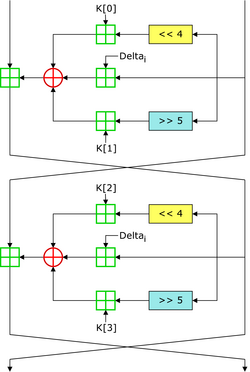
\includegraphics[scale=0.7]{TEA.png}
\caption{Two Feistel rounds (one cycle) of TEA \citep{tea_diagram} }
\label{fig:tea_diagram}
\end{figure}

We know from the answer 3a that,

$L_2$ = ($L_0$ $\boxplus$ ((($R_0$ $\ll$ 4) $\boxplus$ $K_0$) $\oplus$ (($R_0$ $\gg$ 5) $\boxplus$ $K_1$) $\oplus$ ($R_0$ + $\delta_1$)))

As we have access to cipher-texts of the messages of our choice, we know the values of $L_2$, $L_0$ and $R_0$, replacing those values by constants we get the equation of 

$C_2$ = ($C_0$ $\boxplus$ (($C_1$ $\boxplus$ $K_0$) $\oplus$ ($C_2$ $\boxplus$ $K_1$) $\oplus$ $C_3$))

or, $C_4$ = ($C_1$ $\boxplus$ $K_0$) $\oplus$ ($C_2$ $\boxplus$ $K_1$)

From the above equation we can guess the values of $K_0$, $K_1$ and try those values in another equation derived from a new plaintext and ciphertext pair. Since each key is 32bit, we may need $2^{32}$ guesses to solve $K_0$, $K_1$.

Following the above technique, we will need another $2^{32}$ guesses to solve $K_2$, $K_3$.

In conclusion, if a user is allowed to mount a plain-text attack in a 2-round version of TEA, they can derive the value of keys in 2.$2^{32}$ = $2^{33}$ iterations.


\item \textbf{Would the answer described above change if the 4-round version of TEA is used instead?
Justify your answer.}

With the 4-rounds version, the complexity will change exponentially. With 2 Feistel rounds, we have 2 unknown K variables in the equations (i.e. $C_4$ = ($C_1$ $\boxplus$ $K_0$) $\oplus$ ($C_2$ $\boxplus$ $K_1$)). But 4-round equations will involve 4 unknown variables: $K_0$, $K_1$, $K_2$ and $K_3$, which means the number of guesses required will be significantly higher. If we visualize this, we have to plot the data point obtained from multiple plaintext-ciphertext pairs in 4-Dimensions space where axes are $K_0$, $K_1$, $K_2$ and $K_3$. Comparatively, for 2-rounds equations, we will create 2 graphs in 2-dimension space consisting of $K_0$, $K_1$ and $K_2$, $K_3$.

\end{enumerate}

\section{Question}
Read about AES-NI and research its use in programs.

\begin{enumerate}[label=\alph*]

\item \textbf{Determine a way to use hardware accelerated AES in one programming language. Provide a segment of code to encrypt one block (16 bytes) of plaintext using AES hardware instructions such as aesenc, aesenclast, etc. Assume that the plaintext is initially stored in a binary buffer (array) and a 128-bit key is also stored in a binary buffer. Executing your code segment should result in a 16-byte cipher block.}

\begin{minted}
[
frame=lines,
framesep=2mm,
baselinestretch=1.2,
bgcolor=LightGray,
fontsize=\footnotesize,
linenos
]
{c}

#include <stdio.h>
#include <stdint.h>         
#include <wmmintrin.h>  //AES-NI intrinsics library




static __m128i key_expansion(__m128i key,__m128i generated_key){

    generated_key = _mm_shuffle_epi32(generated_key, _MM_SHUFFLE(3,3,3,3));
    key = _mm_xor_si128(key, _mm_slli_si128(key, 4));
    key = _mm_xor_si128(key, _mm_slli_si128(key, 4));
    key = _mm_xor_si128(key, _mm_slli_si128(key, 4));
    return _mm_xor_si128(key, generated_key);
}

static void printOutput(uint8_t *val){
    for (int i = 0; i < 16; ++i)
    {
        printf("0x%x ", val[i]);
    }
}


int main(void){

    uint8_t plainText[] =   {0x32, 0x43, 0xf6, 0xa8, 0x88, 0x5a, 0x30, 0x8d, 0x31, 0x31, 0x98, 0xa2,
                            0xe0, 0x37, 0x07, 0x34};
    uint8_t enc_key[] = {0x2b, 0x7e, 0x15, 0x16, 0x28, 0xae, 0xd2, 0xa6, 0xab, 0xf7, 0x15, 0x88, 0x09,
                            0xcf, 0x4f, 0x3c};
    uint8_t computed_cipher[16];



    
    /*
    *	Key Scheduling is being performed here
    *	Expansion of given cipher key into 11 128 bit partial keys
    *	used in one initial round, 9 main rounds and one final round
    */

    __m128i key_schedule[11];
 
    key_schedule[0] = _mm_loadu_si128((const __m128i*) enc_key);
    key_schedule[1]  = key_expansion(key_schedule[0], _mm_aeskeygenassist_si128(key_schedule[0], 0x01));
    key_schedule[2]  = key_expansion(key_schedule[1], _mm_aeskeygenassist_si128(key_schedule[1], 0x02));
    key_schedule[3]  = key_expansion(key_schedule[2], _mm_aeskeygenassist_si128(key_schedule[2], 0x04));
    key_schedule[4]  = key_expansion(key_schedule[3], _mm_aeskeygenassist_si128(key_schedule[3], 0x08));
    key_schedule[5]  = key_expansion(key_schedule[4], _mm_aeskeygenassist_si128(key_schedule[4], 0x10));
    key_schedule[6]  = key_expansion(key_schedule[5], _mm_aeskeygenassist_si128(key_schedule[5], 0x20));
    key_schedule[7]  = key_expansion(key_schedule[6], _mm_aeskeygenassist_si128(key_schedule[6], 0x40));
    key_schedule[8]  = key_expansion(key_schedule[7], _mm_aeskeygenassist_si128(key_schedule[7], 0x80));
    key_schedule[9]  = key_expansion(key_schedule[8], _mm_aeskeygenassist_si128(key_schedule[8], 0x1B));
    key_schedule[10] = key_expansion(key_schedule[9], _mm_aeskeygenassist_si128(key_schedule[9], 0x36));




    /*  Encyption process starts here */
    

    __m128i state_array = _mm_loadu_si128((__m128i *) plainText);


    /*  Initial round */

    state_array = _mm_xor_si128(state_array, key_schedule[ 0]); 

    /* 	
    *	9 main rounds
    *	each round consists of 4 operations: SubBytes, ShiftRows, MixColumns, AddRoundKeys
    *	using _mm_aesenc_si128 we are performing these 4 operations in one instruction 
    */
    
    for (int i = 1; i < 10; ++i){
    
    	state_array = _mm_aesenc_si128(state_array, key_schedule[i]);
    }
    
    /* 
    *	Final round consists of 3 operations: SubBytes, ShiftRows, AddRoundKeys
    *	using _mm_aesenclast_si128 we are performing these 3 operations in one instruction 
    */

    state_array = _mm_aesenclast_si128(state_array, key_schedule[10]);

    _mm_storeu_si128((__m128i *) computed_cipher, state_array);

    
    printOutput(plainText);	
    printf("\n");
    printOutput(computed_cipher);


    return 0;
}

\end{minted}

\begin{figure}[h!]
\centering
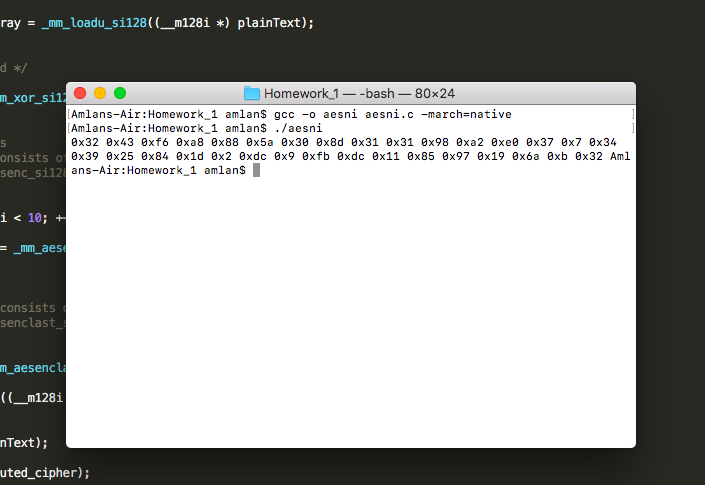
\includegraphics[scale=0.5]{4a_output.png}
\caption{AES-NI program output: Given plain text and computed cipher text}
\label{fig:aesni_output_in_c}
\end{figure}

\newpage
\item \textbf{Is hardware accelerated AES available in all programming languages? Explain.}

Currently, only languages which support hardware accelerated AES are C/C++. Most of the high-level programming languages restrict users from using SIMD directly. C\# provides partial SIMD support with Mono framework and languages like Java, Python, Ruby does have libraries which are just an abstraction layer on top of C implementations. Some of them have plans to implement SIMD in the future whereas most of them stand against implementing this to provide security and stability.
So at the moment, the only way to take full advantage of AES hardware acceleration is using C/C++.

\item \textbf{List resources that were useful in working on this problem.}

Below resources helped me to work on the problem:

\begin{itemize}


\item Computer Security: Principles and Practice (3rd Edition) \citep{compsec_wl}

\item Intel® Advanced Encryption Standard Instructions (AES-NI) \citep{intel_aes}

\item Network  security-  aes  (advanced  encryption  standard)  algorithm Algorithm \citep{aes_utube_sundeep}


\item AES Rijndael Cipher - Visualization \citep{aes_utube_flash}

\item Playing with AES intrinsics \citep{vincent_intrinsics}


\item Using Intel AES-NI and c++ threads to search an AES128 key \citep{aes_github}

\item High-Level Programming Languages Should Improve Support for SIMD Instructions \citep{gaston_simd}

\end{itemize}

\end{enumerate}


\section{Question}

\begin{enumerate}[label=\alph*]

\item \textbf{Find an alternative implementation of AES in the form of a cryptographic library, preferably
one that doesn’t use AES-NI. Write a very small program using that library for accomplishing the task of the previous problem using that library, i.e., for encrypting a 1-block message with a 128-bit key in the ECB mode. Submit the name of the library, the programming language that you used (it can be different from the language
in problem 4), and the code.}

For implementing AES I have used Java as the programming language. It has in-build extensive support for Cryptography. Crypto library from Javax package proved useful to implement this.

\begin{minted}
[
frame=lines,
framesep=2mm,
baselinestretch=1.2,
bgcolor=LightGray,
fontsize=\footnotesize,
linenos
]
{java}

import javax.crypto.Cipher;
import javax.crypto.spec.SecretKeySpec;

public class AES {

    private static SecretKeySpec secretKey;
    
    private static final byte[] plainText = { (byte) 0x32, (byte) 0x43, (byte) 0xf6, (byte) 0xa8, 
                (byte) 0x88, (byte) 0x5a, (byte) 0x30, (byte) 0x8d, (byte) 0x31, (byte) 0x31,
                (byte) 0x98, (byte) 0xa2, (byte) 0xe0, (byte) 0x37, (byte) 0x07, (byte) 0x34 };

    private static final byte[] encKey = { (byte) 0x2b, (byte) 0x7e, (byte) 0x15, (byte) 0x16, 
                (byte) 0x28, (byte) 0xae, (byte) 0xd2, (byte) 0xa6, (byte) 0xab, (byte) 0xf7,
                (byte) 0x15, (byte) 0x88, (byte) 0x09, (byte) 0xcf, (byte) 0x4f, (byte) 0x3c };



    public static void printOutput(byte[] bytes) {
        StringBuilder sb = new StringBuilder();
        sb.append("[ ");
        for (byte b : bytes) {
            sb.append(String.format("0x%02X ", b));
        }
        sb.append("]");
        System.out.println(sb.toString());
    }


    public static void main(String[] args)
    {

        byte[] computedCipher = null;

        try
        {
            secretKey = new SecretKeySpec(encKey, 0,16,"AES");

            Cipher cipher = Cipher.getInstance("AES/ECB/noPadding");
            cipher.init(Cipher.ENCRYPT_MODE, secretKey);
            computedCipher = cipher.doFinal(plainText);
        }
        catch (Exception e)
        {
            System.out.println("Error: " + e.toString());
        }

        printOutput(plainText);
        printOutput(computedCipher);

    }
}

\end{minted}

\begin{figure}[h!]
\centering
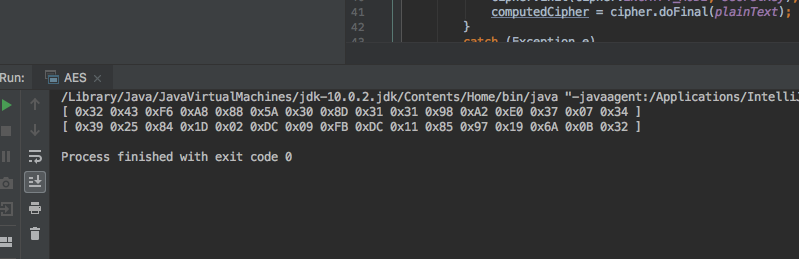
\includegraphics[scale=0.5]{5a_output.png}
\caption{AES program output: Given plain text and computed cipher text}
\label{fig:aes_output_in_java}
\end{figure}

\item \textbf{
Compare the speed of the two implementations. For improved accuracy, run each program to encrypt 1000 1-block messages and report the total time for each of the two programs. If key expansion uses separate code, execute key expansion once followed by 1000 1-block encryptions. Report the times for both implementations and comment on the differences or similarities and any performance conclusions that you can provide.}
\end{enumerate}

\begin{figure}[h!]
\centering
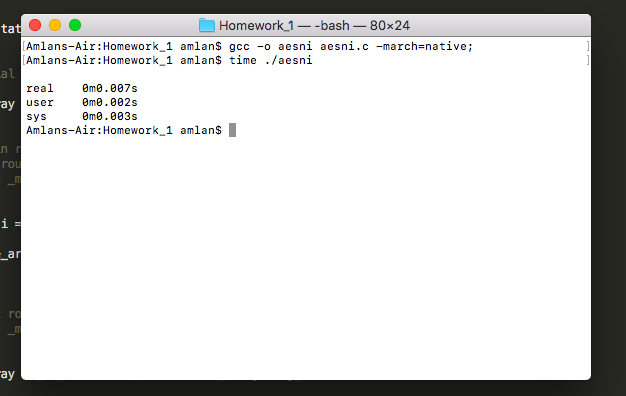
\includegraphics[scale=0.5]{c_exe_time.png}
\caption{AES-NI C program execution time for 1000 1-block encryptions}
\label{fig:c_execution_time}
\end{figure}

\begin{figure}[h!]
\centering
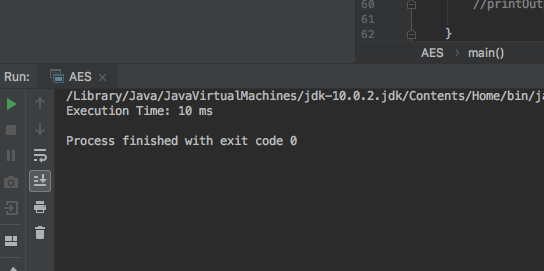
\includegraphics[scale=0.5]{java_exe_time.png}
\caption{AES Java program execution time for 1000 1-block encryptions}
\label{fig:java_execution_time}
\end{figure}

From the above-mentioned reports, we can understand that doing the encryption using AESNI is faster than AES. The difference becomes more evident with a bigger dataset (i.e. For 10000 1-block encryptions, the duration of runtime is 14 and 62 milliseconds respectively). Though there is some overhead due to the choice of programming languages and environments, the difference in performance is quite evident.


\bibliographystyle{unsrt}
\bibliography{references}
\end{document}
